\documentclass{report}
\usepackage{graphicx}
\begin{document}

%-------------------------------------------------------------------------------
%    TITLE PAGE
%-------------------------------------------------------------------------------

\begin{titlepage}
\newcommand{\HRule}{\rule{\linewidth}{0.5mm}}
\center
\textsc{\LARGE Imperial College London}  \\[0.5cm]
\textsc{\Large Department of Computing}  \\[0.5cm]
\textsc{\large Third Year Individual Project} \\[1.5cm]
\HRule \\[0.3cm]
{\huge \bfseries LOST: \\[0.2cm] The Logic Semantics Tutor} \\[0.3cm]
\HRule \\[1.5cm]

% author and supervisors
\begin{minipage}{0.4\textwidth}
\begin{flushleft} \large \emph{Author:} \\
 Alina  \textsc{Boghiu}
\end{flushleft}
\end{minipage}~
\begin{minipage}{0.4\textwidth}
\begin{flushright} \large \emph{Supervisor:} \\
 Ian \textsc{Hodkinson}
\end{flushright}
\begin{flushright} \large \emph{Second marker:} \\
 Fariba \textsc{Sadri}
\end{flushright}
\end{minipage}\\[4cm]
{\large \today}\\[3cm]
\vfill
\end{titlepage}

%-------------------------------------------------------------------------------
%    ABSTRACT
%-------------------------------------------------------------------------------

\begin{abstract}
The aim of this project was to develop a software tool that can teach the 
semantics of first order predicate logic to students by helping them visualise 
the process of sentence evaluation. Thus, the focus was on developing an 
intuitive and engaging user interface to show and allow modification of 
structures, signatures and sentences, as well as provide relevant exercises for 
the student to practice with. The latter is arguably the most important feature 
of this tool and an addition to the functionality of the previous LOST. The user
can now ask to solve 3 automatically generated types of puzzles, within a 
tutorial environment that measures their progress. Completing each lesson is an 
actual achievement and provides real confirmation of understanding the semantics
of first order logic. \\ \\
For robustness, the tool is linked to a lesson database which can be accessed by
students and lecturers alike. The former also have permissions to add, edit or
remove lessons and see their student's progress. \\ \\
I believe these are firm grounds for many possible extensions (such as a
Hintikka game) and can be of real use, standalone or alongside the first year
predicate logic course. This report will provide further detail of its 
implementation and purpose.
\end{abstract}

%-------------------------------------------------------------------------------
%    ACKNOWLEDGEMENTS
%-------------------------------------------------------------------------------

\subsection*{\centering Acknowledgements}
I would like to express gratitude and appreciation to my supervisor, \emph{Ian 
Hodkinson}, for his continuous support and motivation that have guided me 
towards completing this project, as well as to my second marker, \emph{Fariba
Sadri}, for her useful remarks and suggestions.\\ \\
Altogether, the resources, staff and students of the Department of Computing 
have made working on this project enjoyable every day.

%-------------------------------------------------------------------------------
    \tableofcontents
%-------------------------------------------------------------------------------

%-------------------------------------------------------------------------------
%   INTRODUCTION
%-------------------------------------------------------------------------------

\chapter{Introduction}

LOST stands for LOgic Semantics Tutor and aims at providing students with a helpful tool for learning the semantics of first order predicate logic.

\section{Motivation and relevance}
First order logic is a powerful tool, of great importance in computing, mathematics and really any system relying on proofs. For students it is a way of practising and developing important logical skills, it provides a formal mean for studying and understanding common mathematical structures and it forms a rigorous mind. However it is difficult for most students to learn the semantics of first order logic and with this being the key to assigning a truth value to any first-order logical sentence, the issue is important. This project attempts to provide a simple software solution and a solid base for future extensions. \\ \\
On the current market, there are a considerable number of tools designed to help teach natural deduction or equivalences, but very few attempts have been made to design something that will accompany the student in learning the semantics of first order logic and even fewer of them are free. Feedback is currently restricted to lectures and tutorials which means this kind of instant guidance provided by computer software would make a great impact in the way students learn, improving both their and the teacher's experience. Designing such a tool raises interesting questions of what would make an interface intuitive and what does it need to provide the user with, such that they can learn and experiment with the semantics of first order predicate logic.

\section{A brief, non-technical description}
After a bit of thought and research into current solutions, I realised it would not be easy to implement in an attractive way and this will become more obvious after discussing the existing work. Thus one of my guidelines shaped up to be engaging the student as much as possible which software can do if it is intuitive, bug free and most importantly rewarding. The first of these would be achieved if the user is allowed to naturally interact with the application. Because in reality no one likes to read manuals, I aimed to make my program safe to use with a ``click and see what happens'' approach. This required reasoning about as many occurable events and exceptions as possible. As for the actual content point of view, it would be useful if the user could visualize structures in such a way that they could easily guess the meaning of a possible sentence within it. They should be able to use a toolbox-like signature representation to add and remove objects and relations as well as have a way of introducing and evaluating sentences. At this point it became clear that the interface would have three main aspects to handle: structures, signatures and sentences, which will be discussed further in the implementation details section. \\ \\
Next, I aimed for a solid back end that could handle even a completely different interface implementation. This meant for it to be able to correctly evaluate the semantics of a logic formula given a structure, regardless of the input or output method. Parsing the input sentence (be it from a terminal or a GUI) would therefore have to be done reliably and its representation in memory be clear, effectively accessible and easy to evaluate. \\ \\
Features described so far would constitute a minimum viable product, however making it such that the student feels their time was spent worthily was just as important. I aimed to achieve this by implementing a simple quiz system with the possibility of further development. This particular functionality would provide the confirmation a student needs when asked to learn anything.

\section{Report Overview}
In the following chapters the reader can expect a walk through the process of developing the final product, from gathering background information to implementation details, testing procedures and, an as much as possible honest evaluation of the outcome. Though previous knowledge of first order predicate logic and Java would help in understanding the effort that went into this project and its relevance, it is not compulsory. I will revise the essential aspects of the theoretical side, however basic knowledge of logic operators and their meaning (i.e.\ and, or, implies etc.) is assumed.

%-------------------------------------------------------------------------------
%   BACKGROUND
%-------------------------------------------------------------------------------

\chapter{Background}

\section{First order predicate logic semantics}
In order to understand the product I am aiming for we should first take a look 
at what first order predicate logic is and why its semantics can be tricky. As 
an extension of propositional logic, it expresses statements such as 
\emph{Socrates is a man} in much more detail.
While propositional logic would regard this sentence as atomic and simply assign
it a truth value, predicate logic provides a way of describing its internal
structure and of evaluating it within a relevant context. I will use this
sentence to briefly introduce the key concepts used in predicate logic to make
``splitting the atom'' possible. These are:
  \begin{itemize}
	\item \emph{Constants} 
  - which name the objects inside a context (e.g.\ Socrates). One constant can 
  name exactly one object.
	\item \emph{Relation symbols}
  - which describe properties of the objects they take as arguments or, in the
  case of nullary relations (which take no arguments), general properties of
  the structure (e.g.\ \emph{man} is a unary relation, it represents a property
  that Socrates may or may not have).
  \end{itemize}
In order to keep track of these two new concepts, we use a \emph{signature}.
This represents the syntactic side of evaluating a sentence and provides the
necessary tools: constant names and relations symbols. For a computer scientist 
it may be easier to look at it as a collection of abstract classes that can be 
instantiated to form the structure and give it meaning. \\ \\
Using just these concepts, we can now rewrite the sentence we discussed as 
\emph{man(Socrates)}. However we still cannot decide its truth value and at this
point two questions arise: 
First, which is the object that Socrates describes?
Second, what does it mean for something to be a man? \\ \\
This is where the \emph{structure} comes in. It is defined to be a non-empty set of objects that the signature knows about. If we take our structure to be an
imaginary world of hobbits and name one of them Socrates, our sentence would be
false, as Socrates would not be a man, he would be a hobbit. However in the 
context of the real world where Socrates names the famous philosopher, the 
sentence is true. \\ \\
Next, if we want to express something like \emph{All men are mortal} we must 
introduce the two quantifiers. Again, these can be viewed as a way to iterate 
over the objects that form a structure. These are:
	\begin{itemize}
	\item \emph{$\exists$ (Exists)} 
  - which checks that there is at least one object in the structure that
  satisfies the sentence it refers to and makes it true.
	\item \emph{$\forall$ (For all)}
  - which checks that all of the objects in the structure satisfy the sentence 
  it refers to and each make it true.
	\end{itemize}
The sentence can now be written as
\emph{$\forall$(men(x) $\rightarrow$ mortal(x))}
and we refer to x as a bound variable because it is pinned down by a quantifier,
in this case $\forall$. A more precise reading of the above formula would be:
"If something is a man than it is mortal." \\ \\
Another aspect that the user must understand is that sentences containing 
unbound variables are also valid but cannot be evaluated to a truth value. 
Saying "men(x) $\rightarrow$ mortal(x)" makes no sense until we decide what x 
refers to. If x were a constant than it would refer to the object it names, 
however common practice dictates that we reserve the last letters of the 
alphabet for naming variables. It is this kind of subtlety that I am hoping
to make clearer with the help of an interface which shows exactly which objects
are named by constants and which can only be referred to by using quantified 
variables. \\ \\
The theoretical side is obviously what forms the base of this project. It is therefore natural that the implementation follows its key aspects: the strucutre, the signature and the logic formulas. Throughout the report I will inevitably make references to the concepts summarised in this section whilst possibly making further additions and clarifications.

\section{Existing solutions}
As mentioned before, previous attempts have been made to provide software solutions to teaching predicate logic semantics. In fact one student provided a solution for this same project specification in 2007. Furthermore, the Openproof Project at Stanford's Center for the Study of Language and Information (CSLI) is concerned precisely with the application of software in logic and they have developed Tarski's World for this purpose.

\subsection{LOST 2007}
This application was previously available on the DoC's lab machines. Currently however, the only available resource is the user manual. As it is a solution to the same project specification I have carefully studied it and picked up what I thought were several good ideas, whist taking note of things I should avoid. \\ \\
The application provides a good representation of the logical structure. It displays objects as circles, filled with colours corresponding to the unary relation symbols that apply. Binary relation symbols are represented as arrows, also colour coded. The user can drag objects to rearrange them as he seems fit. This representation is quite clear and easy to interpret. For this reason my own implementation is similar, with a few changes aimed at smoothing the experience even further. First I decided objects should have a clear base colour displaying only their name in the case of constants. Then, according to which unary relations apply to it, coloured borders would be added or removed. This eliminates the risk of a confusing pie chart when an object has many relations referring to it. Next, the arrows would be labelled with a list of names of the relations they represent, such that if multiple relations exist amongst two objects there is no need for multiple arrows rendering better space efficiency.\\ \\
Furthermore the application allows the user to interact with the structure with several buttons, a signature tree and a number of forms for creating structures and introducing formulas for evaluation. These are offered to the user according to their intention. The general purpose of all this is important and the functionality essential to the application. However in my own implementation I tried to minimise the number of buttons and additional windows or forms, keeping it simple and in one place. \\ \\
Finally the application offers the possibility to play a Hintikka game, which is a wonderful way of practising logic semantics skills. It also makes an attempt at logic to English translation. These would make very useful extensions to my own application as I chose to focus on the tutorial aspect.

\subsection{Tarski's World}
The Tarski's World application is based on the same principle. Its representation of the structure is a 3D world of blocks. It uses an interpreted first-order language which allows users to write sentences about the world and evaluate their truth. A Henkin-Hintikka game is also provided, along side the main game which consists of questions about the active sentences. This was useful when implementing my own tutorial questions. \\ \\
My single reservation was once more the number of menus, panels and buttons that can become quite irritating since only a few are truly relevant and most don't seem worth the effort of figuring out. From the point of view of a student this can be quite off putting and might drive them towards the classic pen and paper approach. Otherwise it is generally very professionally made and I didn't encounter any major flaws. The learning experience is complete if we take into account the extensions including text books and an online evaluation system that grades the student's performance which I particularly appreciated.

\section{Ideas shaping the final approach}
After looking into the above mentioned solutions and others similar to them it became obvious that the main difficulty with providing a teaching tool for logic semantics is in fact teaching the student to use it. When working with these tools I got the feeling they let the back end lead the implementation of the interface instead of using the latter to hide the inner works. For example, just because there are say 20 relation symbols active in the signature doesn't mean the user wants to see them at all times in a big grid of buttons that takes up half of the work space. I believe it is important to let the user focus on semantics without having to worry too much about the syntactic aspect, which should be provided and hidden as much as possible. \\ \\
Another remark should be made on the tendency of developers to forget the user doesn't know as much as they do. It is impossible to develop a teaching tool without understanding first order predicate logic inside out, which makes it is even harder to empathise with a student that is just starting to learn it. It is therefore easy to unconsciously overestimate the user's knowledge and forget to provide explanations that might in fact be useful to them. For example it might seem counter intuitive that a sentence such as man(Socrates) is false. But if the signature's only unary relation symbol is \emph{hobbit} this may seem obvious to a logician. However the user who tried to input the above sentence might benefit from a message such as ``The unary relation symbol man is not defined in this structure'', instead of their sentence just being rejected as invalid. \\ \\
Finally, I fixed the two features that would make this project unique. First of all I would keep it as simple as possible, making it a priority to minimise the number of buttons and choices the user has to make. This had to be done without sacrificing any of the essential functionality. Secondly, I would make it rewarding, by giving the user an opportunity of testing their skills. As several students have worked on this project specification across the years, I figured this would be a useful and fresh addition.

\section{Software choices}
Having sufficiently stressed the importance of the interface I had to make a choice as to which programming environment would best fit its requirements. I wanted to be able to focus on building something attractive without having to worry too much about the lower level issues like memory assignments, garbage collection or optimal for loop nesting. This, as well as my previous programming experience, perused me to choose Java and Swing, which proved to be at a high enough level for my interface whilst offering me the freedom to design the back end for the sentence evaluation from scratch. Thus I had complete control and understanding of every step that takes a sentence from it's raw form to an outcome. And understanding made it easier to track bugs, make changes and pursue a steady development. Java also ensures a decent compatibility across computer platforms, has extensive documentation and is a reliable language that addresses a large audience. \\ \\
Of further help with the the interface was the IDE. After starting off with Eclipse, I soon realised the simple task of arranging buttons on the panel was uselessly tedious. So after a little research I chose to use NetBeans for its GUI Builder. It took a bit of getting used to, especially with learning to get around the read-only generated code, but eventually everything proved to be 100\% customisable and certainly worth switching to. Overall this saved me significant time and helped me achieve my desired esthetic standard. \\ \\
Java proved to be the right choice again when it came to writing a parser for the logic formulas. It made it easy to link an automated parser, reducing my task to writing a comprehensive grammar. At this point, another choice was to favour Antlr4 over the previous, better known version. What convinced me was its ability to deal with left recursive grammars. Although removing recursivity is a straight forward algorithm, it makes the grammar quite ugly and a bit more difficult to read. Antlr4 also uses an impressive adaptive parsing strategy, making it significantly more time efficient than its static ancestors.\\ \\
For version control I used Git. It is an easy and reliable way of keeping backups, working remotely, tracking progress and proved essential for a project this size as it happened more than once that I had to revert to previous commits and slowly add in changes to discover bugs. It also proved useful for its branches, allowing me to experiment with external Java packages such as mxgraph.\\ \\
For the report I used LaTeX with Vim, which greatly facilitated the text formating and made it easy to keep track of the different sections. The Unix shell was also of great use with compiling Antlr and LaTeX and using Git as well as with occasional remote connections. Finally, the entire project was developed on a Ubuntu 12.04 system. \\ \\

\section{Software Architecture Design Patterns}
As developing proceeded, the size of the code became overwhelming. The separations packages and classes provided was insufficient. When it came to implementing the smallest changes, dependencies inside the code made it a tedious and time consuming task. Therefore, when the back end was finished and I began developing the user interface, I took a step back and revised some software design patterns, in order to choose a system that would best fit my requirements. \\ \\
It was the \emph{Model-View-Controller} pattern that helped the most. By completely separating the back end from the display I was able to keep better track of the whole picture:
\begin{itemize}
\item Model - this represents everything in the back-end. It handles all the information concerning sentences, signatures, structures and evaluation. 
\item View - this represents the interface. It contains all the component types needed to represent logic objects. It also handles the display layout and appearance and contains the project's main method.
\item Controller - this is the class that links the model to the view. To do this it pairs up logic objects with an appropriate graphical component. It also interprets user input such that it can be sent back to the model for interpretation. 
\end{itemize}
Having separated the information from the representation in this way, it became much easier to change the interface since I no longer had to worry about the compatibility with the model. This was essential as designing the GUI meant repeatedly using the application and applying slight variations to see what would be most comfortable for the user. \\ \\
I also used the \emph{Adaptor} structural design pattern, which allowed me to separate the parser generating from the sentence structure. I then used an the Sentence class constructor to convert the parse tree into my own logic tree, which I had designed with an integrated evaluator. \\ \\

%-------------------------------------------------------------------------------
%   MAIN BODY
%-------------------------------------------------------------------------------

\chapter{Approach and Implementation details}

This logic semantics tutoring tool is naturally shaped around the theoretical elements that provide logic formulas with meaning. It contains three packages which I will discuss in the same order they were developed:
\begin{itemize}
\item Evaluator - that holds the logic tree structure along with an adaptor for the parse tree and an evaluator.
\item Parser - which handles the translation of raw logic formulas input as strings into a parse tree.
\item GUI - which contains the user interface and controller.
\end{itemize}

\section{Evaluator}
As it can be deducted from the brief description above, this is the main and largest part of the software. I will start with how logic formulas are supported then move onto the evaluation process and finally the adaptor. \\ \\
The starting point of my project was representing sentences in an efficient computer readable format. It was also important to remain close to a human friendly representation. The solution came once from logic theory, where sentences are often represented with the help of logic trees. These trees have logic operators or quantifiers for nodes and simple atomic formulas for leaves. For example, the sentence \emph{$\forall$(men(x) $\rightarrow$ mortal(x))} is represented by the following tree:

\begin{figure}[h!]
\centering 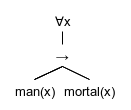
\includegraphics{mortal.png}
\end{figure}
\newpage \noindent
So with this in mind the first step was to build the classes to represent the logic elements that would be used to form the nodes of the logic tree.

\begin{itemize}
\item NullaryRel, UnaryRel, BinaryRel \\
Classes to represent relations symbols with arities from 0 to 2. Although it is possible to have higher arities they are not common in predicate logic and would over complicate the representation too much. Once a stundents understands these three, relations of higher arities are merely an inductive step away.
\item Term \\
A class to represent the parameters relation symbols take. It has a name and is extended by Constant and Variable. The latter adds boolean fields indicating whether it is bound by a certain quantifier. 
\item BinOp \\
An enum type containing all the binary logic operators along with definitions of their behaviour (i.e.\ functions overriding the abstract function evaluate).
\end{itemize}

\subsection{Logic Tree}
Next I build the actual nodes. Each extend the abstract LogicTreeNode class, overriding the evaluate function and providing a pointer to the next node (or nodes in the case of binary operators). They are of course encapsulated by a LogicTree class which has the head of the tree to nicely call evaluate upon. Let us see how each node works in decreasing order of their complexity:

\begin{itemize}
\item ForAllNode\\
This node's evaluation function returns the boolean value representing whether each of the objects in the structures make the sentence true. And it is very important to understand the difference between each object making the sentence true and all objects making the sentence true. For example, to verify the sentence \emph{$\forall$x (men(x) $\rightarrow$ mortal(x))} (All men are mortal) we would take each man in turn and verify that he is mortal, disregarding any animals or other things. It would be wrong to first verify that everything is a man and if so, then verify that everything is mortal. Such a sentence would be written as \emph{$\forall$x men(x)$ \rightarrow \forall$x mortal(x)}. To make this even more clear, let us assume the structure contains an immortal man. This would make the first sentence false because not all men are mortal. However in the case of the second sentence, when verifying that everything is a man, we would find that is not true since there are also animals and other things in the structure. And since falsity implying anything is always true, the second sentence is true. Hence the two sentences have different outcomes and mean different things. \\
In order to handle this correctly, the forall node passes an assignment down the tree to be evaluated with the entire sentence in scope. An assignment represents an object from the structure's domain and to build it, the node has a Term field which points to the variable it quantifies. It uses this term to call the Assignment class constructor, then adds the new assignment to an array of assignments as other quantifiers may be encountered along the way. The node passes the assignment down as a parameter to its evaluation method which iterates over all of the objects in turn and only then puts the outcomes together. If all of them verify the sentence then the final result is returned as true, otherwise as false. 
\item ExistsNode\\
This node follows the same principle. The difference is outcomes of each assignment are put together with an or operator, such that as soon as one is found to be true, the evaluation stops and returns true. If however it reaches the end of the structure domain without finding a term to satisfy the sentence, it returns false.
\item BinaryRelNode\\
This is a leaf node class and contains a BinaryRel field that holds all the information about the relation that needs to be interpreted. At this point it must be clarified that there are in fact two abstract evaluation functions as follows:
\begin{verbatim}
abstract boolean evaluate(Signature s, Assignment a);
abstract boolean evaluate(Signature s, Assignment a1, Assignment a2);
\end{verbatim}
This is because an assignment must be duplicated in the case of a binary relation if both its parameters refer to the same variable (e.g $\forall$x loves(x,x)), or, if both arguments are different variables, naturally an assignment is needed for each. \\
In the case of constants things are more straight forward: the method simply checks the sentence for the object named by the constant.
\item UnaryRelNode \\
This node works in the same way, with only one assignment for the relation's single parameter. 
\item NullaryRelNode \\
This node has a NullaryRel field and always return's that relation's boolean value.
\item EqualsNode \\
Athough it may seem like it could be part of the BinOpNode, this node is actually a leaf as the equals operator takes terms as arguments. So really it is more simillar to the BinOpNode. It also requires two assignments in case both arguments are variables and will return weather the two represent the same object.
\item BinOpNode \\
This is an internal node containing one of the types of operators defined in the enum type described before, as well as pointers to the nodes it takes as arguments. Its evaluation function calls the evaluation functions of the these two nodes in the was described by the operator definition. For example AND will make sore both evaluation functions return true.
\item NotNode \\
Also an internal node that points to the rest of the sentence through a LogicTreeNode field and simply returns its negated outcome.
\item TruthNode and FalsityNode \\
These node always return true and false resepctively. They represent leaf nodes.
\item DummyNode \\
This node is used by the adaptor to translate parse trees an will be further discussed in the relevant section.
\end{itemize}

\subsection{Signature}
In order to understand the symbols used in the logic formula, a signature is needed. In a series of ArrayList fields it holds Strings representing names of the Constant, NullaryRel, UnaryRel and BinaryRel instances. In order to fill these in, its constructor takes a signature object as a parameter.\\ \\
The choice for an array list (here and in other classes) was based on the fact that, being based on a dynamically resizeable array, it would greatly facilitate adding and deletion of objects as well as locating and iterating over its elements. \\ \\
Using just the relation symbols' and constants' names it provides another useful check of the formula's syntax before passing it on to the evaluator. If any symbol used in the sentence is missing from the signature and is not a quantified variable, the user will be prompted with the appropriate message. However this will be discussed further in the section regarding interface implementation where the signature's contribution is greater. In the evaluation context its role is simple: it checks that all the symbols used are declared and valid.

\subsection{Structure}
Now that we have seen the representation of a logic formula and signature, we can proceed to understanding the format of the context in which it will be interpreted. Objects constructed by the Structure class are passed as a parameter to the evaluation method such that an interpretation can be made. \\ \\
The fields of this class are array lists of terms and relations. In order to fill them in, the constructor calls a generate method. This in turn uses four enum types with names for constants and the trhee types of relations. Each enum type has a random chooser method to return one of its members. The generate method uses this and ensures no duplicates are allowed into the final content of the structure. It generates a random number of actual terms and relations using the Term, Const, and relation class constructors described before. \\ \\
Every time the program starts up it creates a new structure which the user can modify, thus ensuring a non empty set of elements at all times to remain consistent with the theoretical deffinition. The details of this will be discussed in the user interface section.

\section{Parser}
I have already discussed the choice of Antlr4 for the purpose of parsing a logic formula from plain string input. In order to generate a parse tree, Antlr needs two things: a grammar and lexer rules. \\ \\
\textbf{The grammar} has proved quite tricky to write as I wanted to offer the user as much input freedom as possible. I also managed to preserve the operator precedence such that it would make it easier for the adaptor to interpret the parse tree. The final and best solution was once more the simple one, with the main rule shaping to be comprehensive and easy to read:
\begin{verbatim}
formula
  : TRUTH
  | FALSITY
  | term EQUALS term
  | relation
  | quantifier formula
  | NOT formula
  | formula AND formula
  | formula OR formula 
  | formula IMPLIES formula
  | formula EQUIV formula 
  | LPAREN formula RPAREN
\end{verbatim}
Please refer to the anex for the complete grammar file.

\textbf{The lexer} rules implied making a few decisions as to what the user should be allowed to use for naming the signature elements. For variable names, the general convention is to use letters towards the end of the alphabet, optionally follows by the character s and/or a number (e.g.\ x3). I stuck to this convention, however allowing all letters of the alphabet. The rule is as follows:
\begin{verbatim}
VARIABLE: [a-z] 's'? [0-9]* ;
\end{verbatim}
For naming relation symbols I allowed any combination of characters beginning with a lower case as long as its length is greater than 1 or beginning with an upper case letter in which case its length must only be greater than 0:
\begin{verbatim}
NAME: [A-Z] | [a-zA-Z] [a-zA-Z09'_']+ ;
\end{verbatim}
The lexer ignores white spaces or new line characters:
\begin{verbatim}
WS: [ \t\r\n]+ -> skip ;
\end{verbatim}
Finally, it provides rules for the logic symbol tokens:
\begin{verbatim}
LPAREN   : '('	;
RPAREN   : ')'	; 
AND      : '∧'	;
OR       : '∨'	;
NOT      : '¬'	;
IMPLIES  : '→'	;
EXISTS	 : '∃'	;
FORALL	 : '∀'	;
TRUTH    : '⊤'	;
FALSITY  : '⊥'	;
EQUALS	 : '='	;
EQUIV	   : '↔'	;
\end{verbatim}
Together, the rules above represent the entire lexer file.

\section{Adaptor}
At this point we can return to look at the LogicTree class constructor which works as an adaptor for the parse tree. Antlr provides a user basic interface which can be run from the terminal to visualise this tree. For the sentence \emph{All men are mortal} the following tree will be generated:
\begin{figure}[h!]
\centering 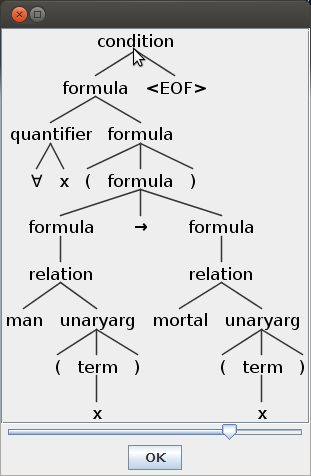
\includegraphics[scale=0.5]{antlr.png}
\end{figure}
Each node is created from one of the parser context classes. 
\begin{verbatim}
folParser$ConditionContext
folParser$FormulaContext
folParser$QuantifierContext
folParser$RelationContext
folParser$BinaryargContext
folParser$UnaryArgContext
folParser$TermContext
\end{verbatim}
The first thing to notice is that the parser will generate a \emph{formula} node that does not correspond a type of logic node but is just a rule that guides the parsing. For this reason I created the dummy node which simply points to the rest of the tree through a LogicTreeNode field and returns that node's outcome without altering it. \\ \\
The adaptor provides a rule of interpretation for each of these classes through a switch statements. The default case is an error message for a complete picture, although it is not reachable, as each node of the parse must be an instance of one of these classes. The constructor performs a breadth first search and generates the appropriate LogicTreeNode for each node in the parse tree. Once finished it returns a pointer to the head of the tree. The sentence is now complete and ready for evaluation.

\section{User Interface}
\subsection{The View}
The layout of the workbench is also designed around the three main elements involved in semantics:
\begin{itemize}
\item Structure panel \\
It is the main working area, taking up most of the upper left side. It displays objects as squares with labels for Constants and colour coded borders to represent unary relations that apply. Binary relations are represented by arrows between objects, also labelled with the list of relations that apply to that arrow. Nullary relations are displayed as a list of labels and can be rearranged to make best use of the space available.
\item Signature panel
It is a tabbed panel at the right side of the workbench, with a tab for each type of element: Constants, nullary, unary and binary relation symbols. Each tab also contains buttons for manipulating their content. 
\item Sentence panel
Situated at the bottom of the window, it provides the means for introducing logic formulas and a scrollable list to store them and their outcome.
\end{itemize}
  \subsection{The Controller}

\section{Exception handling and user guidance}
Even the most intuitive interface needs to be able to guide its user if necessary. This is done with the help of useful error messages and clear, concise instructions.

\subsection{Instructions, tips and tricks}
At the top of the window there is of course a menu bar which provides further assistance for the user. \\ \\

Firstly, it can be used for saving and loading workbenches and their elements.\\
Secondly, it provides a number of tips and tricks to help the user get familiar with the interface.

\subsection{Error messages}
In order to handle bad user input or illegal operations I designed a number of exception classes.

\begin{itemize}
\item DuplicateDefinitionException
\item UnboundException and ThisUnboundException
\item UndefinedRelationException
\end{itemize}

Further error messages are also displayed for inbuilt exceptions:

\begin{itemize}
\item Index out of bounds\\
This can occur when a user presses buttons that require a list element to be selected so that the method can pass down an index. In such cases an error message is displayed only once to instruct the user that they must make a selection.
\item I/O exception\\
This can occur when the user tries to load a corrupted or otherwise inaccessible file. The error message informs accordingly.
\end{itemize}

%-------------------------------------------------------------------------------
%   EVALUATION
%-------------------------------------------------------------------------------

\chapter{Evaluation}
\section{Quantitative evaluation}
\begin{verbatim}
 ∀x(R(Fred,x) →  ∀y(R(x,y) → P(y)))
 ∃x∀y (A ∨ B) ∧ B ∧ ¬D ∧ E ∧ F ∨ G ∨ H
 ∃x∀y (A ∨ B) ∧ B ∨ ¬D ∧ E ∧ F ∨ G ∨ H
 ∃x∀y (A ∨ B) → B ∨ (¬D) ∧ E ∧ (F ∨ G) ∨ H
 A ∨ ¬B ∧ C
 B ∨ (¬D) ∧ E ∨ H ∧ E
 Loves(fred,wilma) ↔ is_in_the_air(love)
 ⊤
 brian = rian
 ∃x∀ys(happy(x) → ¬A)
 ∀x(Red(Fred,x) ∧ E ∧ E ∧ E ∨ H → E →  ∀y(R(x,y) → P(y)))
 A → B → C → D → E (Assumes A → B → C means (A → B) → C)
 A → B → C → (D → E)
 P → (Q ∨ ¬R) ∧ ¬S
 ∀x P(x) → ∃y Q(x,y)
\end{verbatim}

% minimum viable product, robustness, bugs!, testing 
\section{Qualitative evaluation}
 % have I done it well, is it appealing, performant, pretty

%-------------------------------------------------------------------------------
%   CONCLUSIONS AND FUTURE WORK
%-------------------------------------------------------------------------------

\chapter{Conclusions and Future Work}
\section{Learning outcomes}
\section{Potential improvements}
\section{Potential extensions}

%-------------------------------------------------------------------------------
%   BIBIOGRAPHY
%-------------------------------------------------------------------------------

\begin{thebibliography}{9}
%\bibitem{lamport94}
%  Leslie Lamport,
%  \emph{\LaTeX: A Document Preparation System}.
%  Addison Wesley, Massachusetts,
%  2nd Edition,
%  1994.

% Antlr4 documentation
% Java documentation
% Git doc
% Software patterns slides, text book
% Predicate logic slides
% Predicate logic  text book
% Compilers slides
% StackOverflow

\end{thebibliography}

%-------------------------------------------------------------------------------
%   APPENDIX
%-------------------------------------------------------------------------------

\appendix
\chapter{Code UML Diagram}
\chapter{Parser grammar}
\begin{verbatim}
grammar fol ;

condition
  : formula EOF ;

formula
  : TRUTH
  | FALSITY
  | term EQUALS term
  | relation
  | quantifier formula
  | NOT formula
  | formula AND formula
  | formula OR formula 
  | formula IMPLIES formula
  | formula EQUIV formula 
  | LPAREN formula RPAREN ;

term
  : VARIABLE
  | NAME ;

quantifier
  : FORALL VARIABLE
  | EXISTS VARIABLE ;

relation
    : NAME binaryarg
    | NAME unaryarg
    | NAME ;

binaryarg
    : LPAREN term ',' term RPAREN ;

unaryarg
    : LPAREN term RPAREN ;

\end{verbatim}

\chapter{Short demo}

%-------------------------------------------------------------------------------

\end{document}

